\setAuthor{Jaan Kalda}
\setRound{lõppvoor}
\setYear{2015}
\setNumber{G 7}
\setDifficulty{9}
\setTopic{Geomeetriline optika}

\prob{Ring ja ellips}
Juuresoleval joonisel on kujutatud ring ja sellest koondava läätse poolt tekitatud kujutis. Leidke läätse keskpunkt, optiline peatelg ja fookus.
\begin{center}
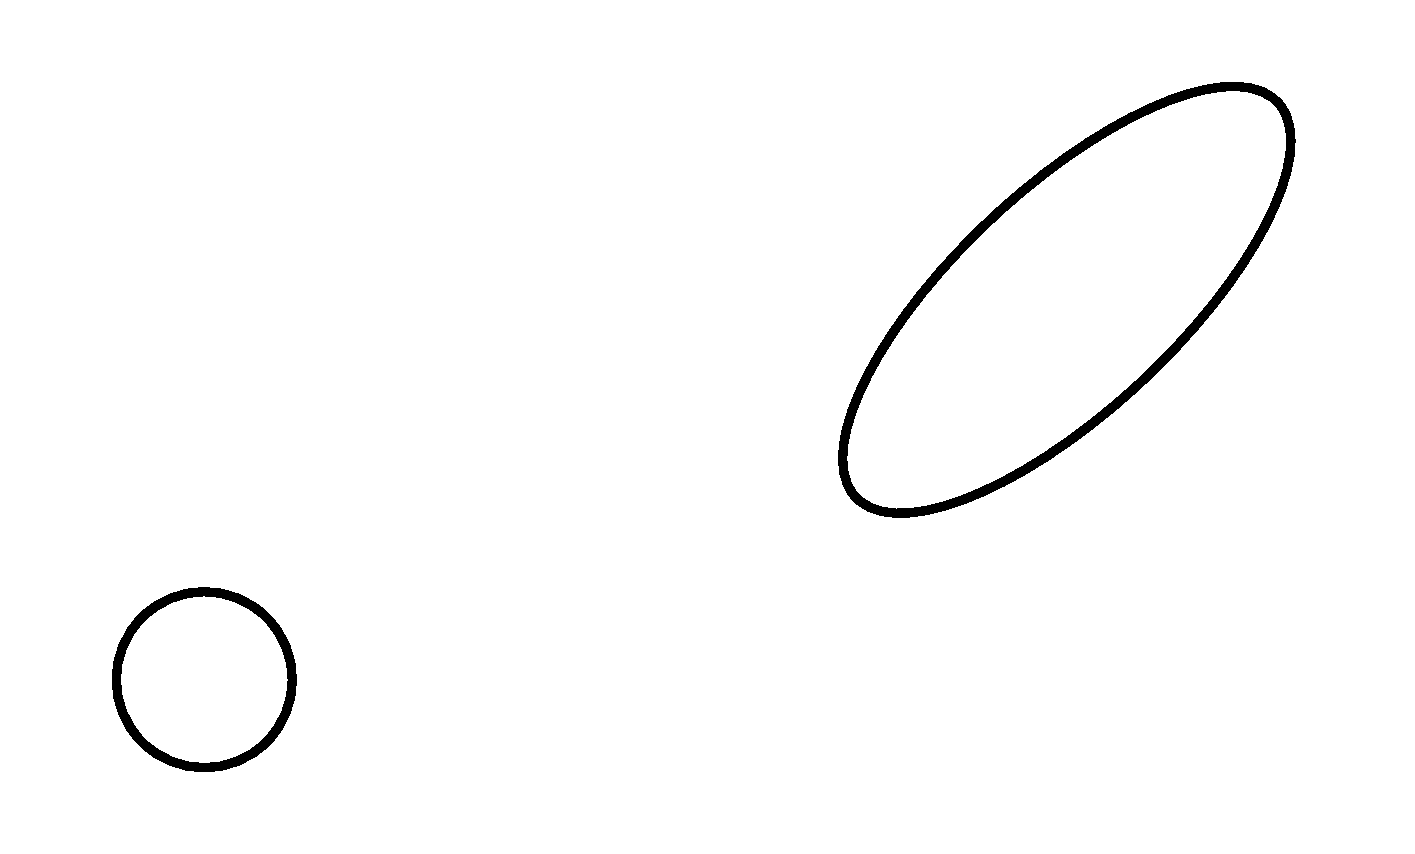
\includegraphics[width=0.7\textwidth]{2015-v3g-07-ringjaellips}%
\end{center}

\hint
Esimesena tuleks alustada läätse keskpunkti leidmisega, seejärel paika panna läätse orientatsioon ning fookus. Keskpunkti leidmiseks tasub vaadata kiiri, mis puutuvad nii ringi kui ka ellipsit.

\solu
Läätse keskpunkt $O$ on ringile ja ellipsile tõmmatud puutujate lõikepunkt, kuna puutepunktid peavad olema originaalkujutise paarid ning neid ühendavad sirged peavad läbima läätse keskpunkti. Läätse tasandi leidmiseks valime ringil kaks punkti, $A$ ja $B$, ning leiame nende kujutised ellipsil $A'$ ja $B'$ sirgete $AO$ ja $BO$ ning ellipsi lõikepunktidena. Kui originaal on ringi kahest lõikepunktist see, mis asub läätsest kaugemal, siis selle kujutis on see, mis on läätsele lähemal (ja vastupidi), sest tõeline kujutis on pööratud tagurpidi. Kiir $AB$ peab murduma läätses kiireks $A'B'$, murdepunkt annab meile punkti $L$ läätsel ning sirge $OL$ on läätse tasandiks. Optilise peatelje $o$ leiame sirgele $OL$ punktist $O$ tõmmatud ristsirgena. Fookuse leidmiseks tõmbame punktist $A$ kiire, mis on paralleelne $o$-ga ja murdub läätsel punkti $A'$ läbivaks kiireks, mille lõikepunkt $o$-ga annab fookuse $F$.

\begin{center}
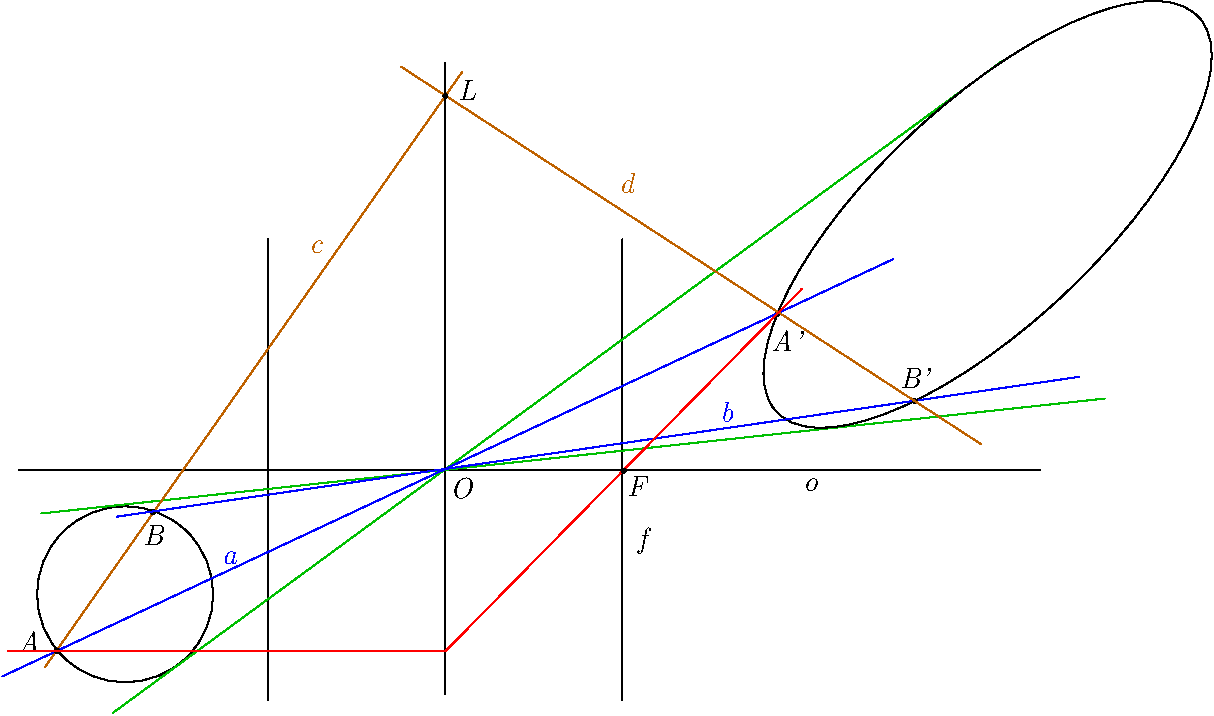
\includegraphics[width=\textwidth]{2015-v3g-07-ellips_lah}
\end{center}

\probeng{Circle and eclipse}
A ring and its image produced by a convex lens are depicted in the figure. Find the center of the lens, the optical axis and the focal point.
\begin{center}
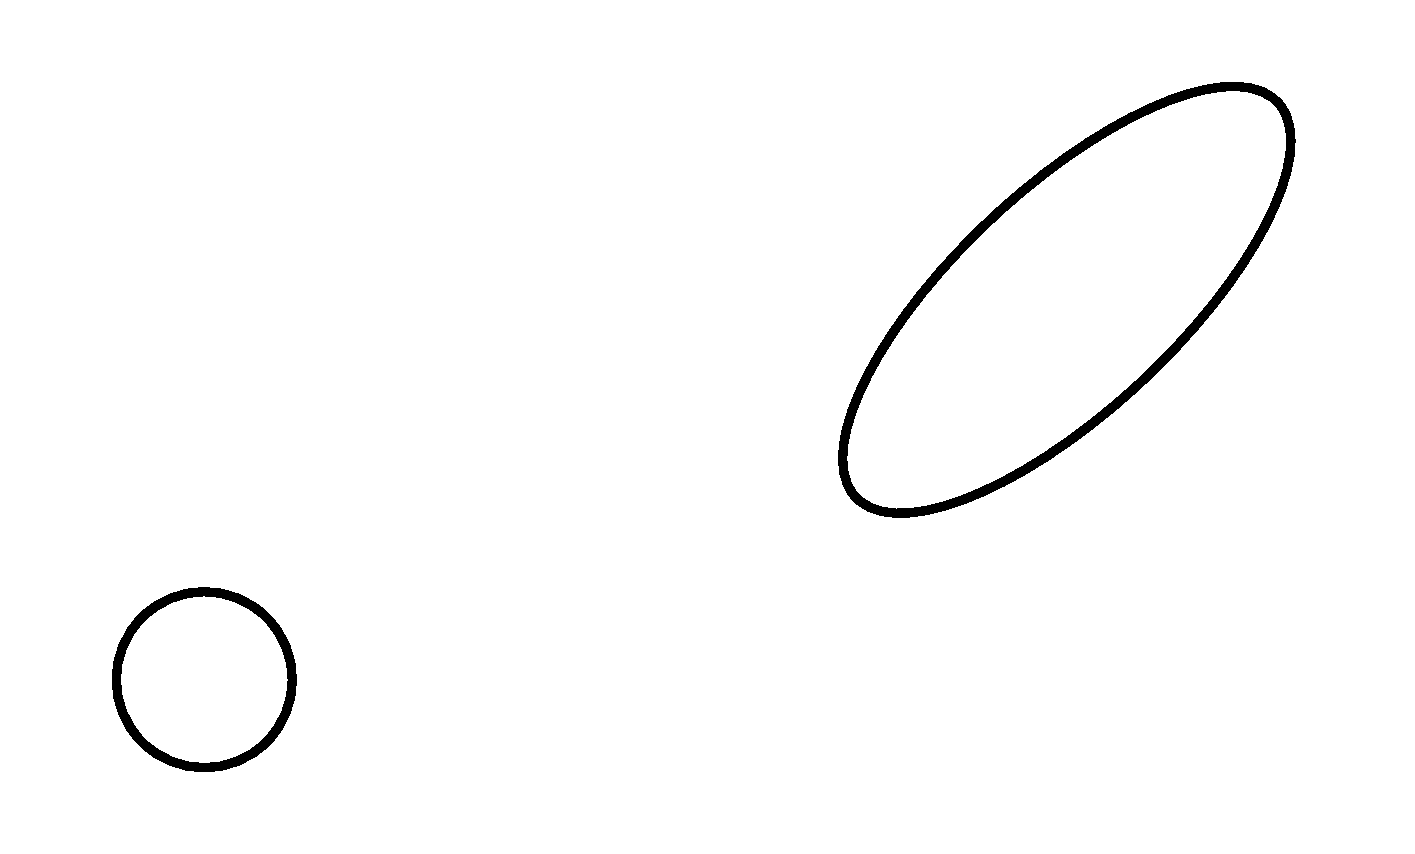
\includegraphics[width=0.7\textwidth]{2015-v3g-07-ringjaellips}%
\end{center}

\hinteng
At first you should find the center of the lens, then its orientation and focal point. To find the center you should observe rays that touch both the ring and the ellipse.

\solueng
The center $O$ of the lens is the intersection point of the tangents drawn from the ring and the eclipse because intersection points have to be in pairs with original images and the lines connecting them have to go through the center. To find the plane of the lens we choose two points on the ring, $A$ and $B$, and we find their images $A'$ and $B'$ on the eclipse to be the intersection points of lines $AO$ and $BO$ and the eclipse. If the original from the two intersection points of the ring is the one that is further from the lens then its image is the one that is closer to the lens (and the other way around), because a real image is turned upside down. The ray $AB$ has to refract in the mirror into the ray $A'B'$, the refraction point gives us a point $L$ on the lens and the line $OL$ is the plane of the lens. We find the optical axis $o$ to be the perpendicular drawn on the line $OL$ from the point $O$. To find the focal point we draw a line from the point $A$ that is parallel to $o$ and refracts into a ray going through the point $A'$. The intersection point of this ray with $o$ gives us the focal point $F$.
\begin{center}
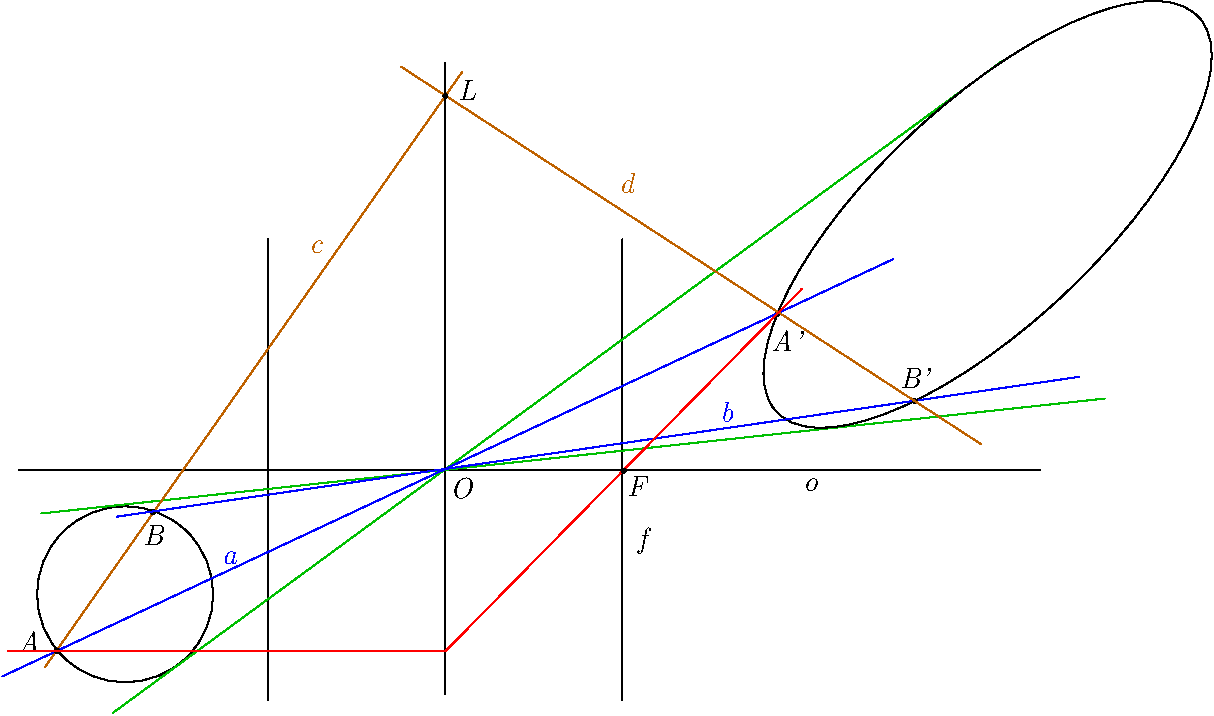
\includegraphics[width=\textwidth]{2015-v3g-07-ellips_lah}
\end{center}
\probend